\documentclass[14pt,russian]{scrartcl}
\let\counterwithout\relax
\let\counterwithin\relax
\usepackage{lmodern}
\usepackage{float}
\usepackage{xcolor}
\usepackage{extsizes}
\usepackage{subfig}
\usepackage[export]{adjustbox}
\usepackage{tocvsec2} % возможность менять учитываемую глубину разделов в оглавлении
\usepackage[subfigure]{tocloft}

\usepackage{fancyvrb}
\usepackage{ulem,bm,mathrsfs,ifsym} %зачеркивания, особо жирный стиль и RSFS начертание
\usepackage{sectsty} % переопределение стилей подразделов
%%%%%%%%%%%%%%%%%%%%%%%

%%% Поля и разметка страницы %%%
\usepackage{pdflscape}                              % Для включения альбомных страниц
\usepackage{geometry}                               % Для последующего задания полей
\geometry{a4paper,tmargin=2cm,bmargin=2cm,lmargin=3cm,rmargin=1cm} % тоже самое, но лучше

%%% Математические пакеты %%%
\usepackage{amsthm,amsfonts,amsmath,amssymb,amscd}  % Математические дополнения от AMS
\usepackage{mathtools}                              % Добавляет окружение multlined
\usepackage[perpage]{footmisc}

%%%% Установки для размера шрифта 14 pt %%%%
%% Формирование переменных и констант для сравнения (один раз для всех подключаемых файлов)%%
%% должно располагаться до вызова пакета fontspec или polyglossia, потому что они сбивают его работу
%\newlength{\curtextsize}
%\newlength{\bigtextsize}
%\setlength{\bigtextsize}{13pt}
\KOMAoptions{fontsize=14pt}

\makeatletter
\def\showfontsize{\f@size{} point}
\makeatother

%\makeatletter
%\show\f@size                                       % неплохо для отслеживания, но вызывает стопорение процесса, если документ компилируется без команды  -interaction=nonstopmode 
%\setlength{\curtextsize}{\f@size pt}
%\makeatother

%шрифт times
\usepackage{tempora}

   %%% Решение проблемы копирования текста в буфер кракозябрами
%    \input glyphtounicode.tex
%    \input glyphtounicode-cmr.tex %from pdfx package
%    \pdfgentounicode=1
    \usepackage{cmap}                               % Улучшенный поиск русских слов в полученном pdf-файле
    \usepackage[T2A]{fontenc}                       % Поддержка русских букв
    \usepackage[utf8]{inputenc}                     % Кодировка utf8
    \usepackage[english, main=russian]{babel}            % Языки: русский, английский
%   \IfFileExists{pscyr.sty}{\usepackage{pscyr}}{}  % Красивые русские шрифты
%\renewcommand{\rmdefault}{ftm}
%%% Оформление абзацев %%%
\usepackage{indentfirst}                            % Красная строка
%\usepackage{eskdpz}

%%% Таблицы %%%
\usepackage{longtable}                              % Длинные таблицы
\usepackage{multirow,makecell,array}                % Улучшенное форматирование таблиц
\usepackage{booktabs}                               % Возможность оформления таблиц в классическом книжном стиле (при правильном использовании не противоречит ГОСТ)

%%% Общее форматирование
\usepackage{soulutf8}                               % Поддержка переносоустойчивых подчёркиваний и зачёркиваний
\usepackage{icomma}                                 % Запятая в десятичных дробях



%%% Изображения %%%
\usepackage{graphicx}                               % Подключаем пакет работы с графикой
\usepackage{wrapfig}

%%% Списки %%%
\usepackage{enumitem}

%%% Подписи %%%
\usepackage{caption}                                % Для управления подписями (рисунков и таблиц) % Может управлять номерами рисунков и таблиц с caption %Иногда может управлять заголовками в списках рисунков и таблиц
%% Использование:
%\begin{table}[h!]\ContinuedFloat - чтобы не переключать счетчик
%\captionsetup{labelformat=continued}% должен стоять до самого caption
%\caption{}
% либо ручками \caption*{Продолжение таблицы~\ref{...}.} :)

%%% Интервалы %%%

%%% Счётчики %%%
\usepackage[figure,table,section]{totalcount}               % Счётчик рисунков и таблиц
\DeclareTotalCounter{lstlisting}
\usepackage{totcount}                               % Пакет создания счётчиков на основе последнего номера подсчитываемого элемента (может требовать дважды компилировать документ)
\usepackage{totpages}                               % Счётчик страниц, совместимый с hyperref (ссылается на номер последней страницы). Желательно ставить последним пакетом в преамбуле

%%% Продвинутое управление групповыми ссылками (пока только формулами) %%%
%% Кодировки и шрифты %%%

%   \newfontfamily{\cyrillicfont}{Times New Roman}
%   \newfontfamily{\cyrillicfonttt}{CMU Typewriter Text}
	%\setmainfont{Times New Roman}
	%\newfontfamily\cyrillicfont{Times New Roman}
	%\setsansfont{Times New Roman}                    %% задаёт шрифт без засечек
%	\setmonofont{Liberation Mono}               %% задаёт моноширинный шрифт
 %   \IfFileExists{pscyr.sty}{\renewcommand{\rmdefault}{ftm}}{}
%%% Интервалы %%%
%linespread-реализация ближе к реализации полуторного интервала в ворде.
%setspace реализация заточена под шрифты 10, 11, 12pt, под остальные кегли хуже, но всё же ближе к типографской классике. 
\linespread{1.3}                    % Полуторный интервал (ГОСТ Р 7.0.11-2011, 5.3.6)
%\renewcommand{\@biblabel}[1]{#1}

%%% Гиперссылки %%%
\usepackage{hyperref}

%%% Выравнивание и переносы %%%
\sloppy                             % Избавляемся от переполнений
\clubpenalty=10000                  % Запрещаем разрыв страницы после первой строки абзаца
\widowpenalty=10000                 % Запрещаем разрыв страницы после последней строки абзаца

\makeatletter % малые заглавные, small caps shape
\let\@@scshape=\scshape
\renewcommand{\scshape}{%
  \ifnum\strcmp{\f@series}{bx}=\z@
    \usefont{T1}{cmr}{bx}{sc}%
  \else
    \ifnum\strcmp{\f@shape}{it}=\z@
      \fontshape{scsl}\selectfont
    \else
      \@@scshape
    \fi
  \fi}
\makeatother

%%% Подписи %%%
%\captionsetup{%
%singlelinecheck=off,                % Многострочные подписи, например у таблиц
%skip=2pt,                           % Вертикальная отбивка между подписью и содержимым рисунка или таблицы определяется ключом
%justification=centering,            % Центрирование подписей, заданных командой \caption
%}
%%%        Подключение пакетов                 %%%
\usepackage{ifthen}                 % добавляет ifthenelse
%%% Инициализирование переменных, не трогать!  %%%
\newcounter{intvl}
\newcounter{otstup}
\newcounter{contnumeq}
\newcounter{contnumfig}
\newcounter{contnumtab}
\newcounter{pgnum}
\newcounter{bibliosel}
\newcounter{chapstyle}
\newcounter{headingdelim}
\newcounter{headingalign}
\newcounter{headingsize}
\newcounter{tabcap}
\newcounter{tablaba}
\newcounter{tabtita}
%%%%%%%%%%%%%%%%%%%%%%%%%%%%%%%%%%%%%%%%%%%%%%%%%%

%%% Область упрощённого управления оформлением %%%

%% Интервал между заголовками и между заголовком и текстом
% Заголовки отделяют от текста сверху и снизу тремя интервалами (ГОСТ Р 7.0.11-2011, 5.3.5)
\setcounter{intvl}{3}               % Коэффициент кратности к размеру шрифта

%% Отступы у заголовков в тексте
\setcounter{otstup}{0}              % 0 --- без отступа; 1 --- абзацный отступ

%% Нумерация формул, таблиц и рисунков
\setcounter{contnumeq}{1}           % Нумерация формул: 0 --- пораздельно (во введении подряд, без номера раздела); 1 --- сквозная нумерация по всей диссертации
\setcounter{contnumfig}{1}          % Нумерация рисунков: 0 --- пораздельно (во введении подряд, без номера раздела); 1 --- сквозная нумерация по всей диссертации
\setcounter{contnumtab}{1}          % Нумерация таблиц: 0 --- пораздельно (во введении подряд, без номера раздела); 1 --- сквозная нумерация по всей диссертации

%% Оглавление
\setcounter{pgnum}{0}               % 0 --- номера страниц никак не обозначены; 1 --- Стр. над номерами страниц (дважды компилировать после изменения)

%% Библиография
\setcounter{bibliosel}{1}           % 0 --- встроенная реализация с загрузкой файла через движок bibtex8; 1 --- реализация пакетом biblatex через движок biber

%% Текст и форматирование заголовков
\setcounter{chapstyle}{1}           % 0 --- разделы только под номером; 1 --- разделы с названием "Глава" перед номером
\setcounter{headingdelim}{1}        % 0 --- номер отделен пропуском в 1em или \quad; 1 --- номера разделов и приложений отделены точкой с пробелом, подразделы пропуском без точки; 2 --- номера разделов, подразделов и приложений отделены точкой с пробелом.

%% Выравнивание заголовков в тексте
\setcounter{headingalign}{0}        % 0 --- по центру; 1 --- по левому краю

%% Размеры заголовков в тексте
\setcounter{headingsize}{0}         % 0 --- по ГОСТ, все всегда 14 пт; 1 --- пропорционально изменяющийся размер в зависимости от базового шрифта

%% Подпись таблиц
\setcounter{tabcap}{0}              % 0 --- по ГОСТ, номер таблицы и название разделены тире, выровнены по левому краю, при необходимости на нескольких строках; 1 --- подпись таблицы не по ГОСТ, на двух и более строках, дальнейшие настройки: 
%Выравнивание первой строки, с подписью и номером
\setcounter{tablaba}{2}             % 0 --- по левому краю; 1 --- по центру; 2 --- по правому краю
%Выравнивание строк с самим названием таблицы
\setcounter{tabtita}{1}             % 0 --- по левому краю; 1 --- по центру; 2 --- по правому краю

%%% Рисунки %%%
\DeclareCaptionLabelSeparator*{emdash}{~--- }             % (ГОСТ 2.105, 4.3.1)
\captionsetup[figure]{labelsep=emdash,font=onehalfspacing,position=bottom}

%%% Таблицы %%%
\ifthenelse{\equal{\thetabcap}{0}}{%
    \newcommand{\tabcapalign}{\raggedright}  % по левому краю страницы или аналога parbox
}

\ifthenelse{\equal{\thetablaba}{0} \AND \equal{\thetabcap}{1}}{%
    \newcommand{\tabcapalign}{\raggedright}  % по левому краю страницы или аналога parbox
}

\ifthenelse{\equal{\thetablaba}{1} \AND \equal{\thetabcap}{1}}{%
    \newcommand{\tabcapalign}{\centering}    % по центру страницы или аналога parbox
}

\ifthenelse{\equal{\thetablaba}{2} \AND \equal{\thetabcap}{1}}{%
    \newcommand{\tabcapalign}{\raggedleft}   % по правому краю страницы или аналога parbox
}

\ifthenelse{\equal{\thetabtita}{0} \AND \equal{\thetabcap}{1}}{%
    \newcommand{\tabtitalign}{\raggedright}  % по левому краю страницы или аналога parbox
}

\ifthenelse{\equal{\thetabtita}{1} \AND \equal{\thetabcap}{1}}{%
    \newcommand{\tabtitalign}{\centering}    % по центру страницы или аналога parbox
}

\ifthenelse{\equal{\thetabtita}{2} \AND \equal{\thetabcap}{1}}{%
    \newcommand{\tabtitalign}{\raggedleft}   % по правому краю страницы или аналога parbox
}

\DeclareCaptionFormat{tablenocaption}{\tabcapalign #1\strut}        % Наименование таблицы отсутствует
\ifthenelse{\equal{\thetabcap}{0}}{%
    \DeclareCaptionFormat{tablecaption}{\tabcapalign #1#2#3}
    \captionsetup[table]{labelsep=emdash}                       % тире как разделитель идентификатора с номером от наименования
}{%
    \DeclareCaptionFormat{tablecaption}{\tabcapalign #1#2\par%  % Идентификатор таблицы на отдельной строке
        \tabtitalign{#3}}                                       % Наименование таблицы строкой ниже
    \captionsetup[table]{labelsep=space}                        % пробельный разделитель идентификатора с номером от наименования
}
\captionsetup[table]{format=tablecaption,singlelinecheck=off,font=onehalfspacing,position=top,skip=-5pt}  % многострочные наименования и прочее
\DeclareCaptionLabelFormat{continued}{Продолжение таблицы~#2}
\setlength{\belowcaptionskip}{.2cm}
\setlength{\intextsep}{0ex}

%%% Подписи подрисунков %%%
\renewcommand{\thesubfigure}{\asbuk{subfigure}}           % Буквенные номера подрисунков
\captionsetup[subfigure]{font={normalsize},               % Шрифт подписи названий подрисунков (не отличается от основного)
    labelformat=brace,                                    % Формат обозначения подрисунка
    justification=centering,                              % Выключка подписей (форматирование), один из вариантов            
}
%\DeclareCaptionFont{font12pt}{\fontsize{12pt}{13pt}\selectfont} % объявляем шрифт 12pt для использования в подписях, тут же надо интерлиньяж объявлять, если не наследуется
%\captionsetup[subfigure]{font={font12pt}}                 % Шрифт подписи названий подрисунков (всегда 12pt)

%%% Настройки гиперссылок %%%

\definecolor{linkcolor}{rgb}{0.0,0,0}
\definecolor{citecolor}{rgb}{0,0.0,0}
\definecolor{urlcolor}{rgb}{0,0,0}

\hypersetup{
    linktocpage=true,           % ссылки с номера страницы в оглавлении, списке таблиц и списке рисунков
%    linktoc=all,                % both the section and page part are links
%    pdfpagelabels=false,        % set PDF page labels (true|false)
    plainpages=true,           % Forces page anchors to be named by the Arabic form  of the page number, rather than the formatted form
    colorlinks,                 % ссылки отображаются раскрашенным текстом, а не раскрашенным прямоугольником, вокруг текста
    linkcolor={linkcolor},      % цвет ссылок типа ref, eqref и подобных
    citecolor={citecolor},      % цвет ссылок-цитат
    urlcolor={urlcolor},        % цвет гиперссылок
    pdflang={ru},
}
\urlstyle{same}
%%% Шаблон %%%
%\DeclareRobustCommand{\todo}{\textcolor{red}}       % решаем проблему превращения названия цвета в результате \MakeUppercase, http://tex.stackexchange.com/a/187930/79756 , \DeclareRobustCommand protects \todo from expanding inside \MakeUppercase
\setlength{\parindent}{2.5em}                       % Абзацный отступ. Должен быть одинаковым по всему тексту и равен пяти знакам (ГОСТ Р 7.0.11-2011, 5.3.7).

%%% Списки %%%
% Используем дефис для ненумерованных списков (ГОСТ 2.105-95, 4.1.7)
%\renewcommand{\labelitemi}{\normalfont\bfseries~{---}} 
\renewcommand{\labelitemi}{\bfseries~{---}} 
\setlist{nosep,%                                    % Единый стиль для всех списков (пакет enumitem), без дополнительных интервалов.
    labelindent=\parindent,leftmargin=*%            % Каждый пункт, подпункт и перечисление записывают с абзацного отступа (ГОСТ 2.105-95, 4.1.8)
}
%%%%%%%%%%%%%%%%%%%%%%
%\usepackage{xltxtra} % load xunicode

\usepackage{ragged2e}
\usepackage[explicit]{titlesec}
\usepackage{placeins}
\usepackage{xparse}

\usepackage{listingsutf8}
\usepackage{url} %пакеты расширений
\usepackage{algorithm, algorithmicx}
\usepackage[noend]{algpseudocode}
\usepackage{blkarray}
\usepackage{chngcntr}
\usepackage{tabularx}
\newcommand*\template[1]{\text{<}#1\text{>}}

  
\titleformat{name=\section,numberless}[block]{\normalfont\Large\centering}{}{0em}{#1}
\titleformat{\section}[block]{\normalfont\Large\bfseries\raggedright}{}{0em}{\thesection\hspace{0.25em}#1}
\titleformat{\subsection}[block]{\normalfont\Large\bfseries\raggedright}{}{0em}{\thesubsection\hspace{0.25em}#1}
\titleformat{\subsubsection}[block]{\normalfont\large\bfseries\raggedright}{}{0em}{\thesubsubsection\hspace{0.25em}#1}

\let\Algorithm\algorithm
\renewcommand\algorithm[1][]{\Algorithm[#1]\setstretch{1.5}}

\usepackage{pifont}
\usepackage{calc}
\usepackage{suffix}
\usepackage{csquotes}
\DeclareQuoteStyle{russian}
    {\guillemotleft}{\guillemotright}[0.025em]
    {\quotedblbase}{\textquotedblleft}
\ExecuteQuoteOptions{style=russian}
\newcommand{\enq}[1]{\enquote{#1}}  
\newcommand{\eng}[1]{\begin{english}#1\end{english}}
% Подчиненные счетчики в окружениях http://old.kpfu.ru/journals/izv_vuz/arch/sample1251.tex
\newcounter{cTheorem} 
\newcounter{cDefinition}
\newcounter{cConsequent}
\newcounter{cExample}
\newcounter{cLemma}
\newcounter{cConjecture}
\newtheorem{Theorem}{Теорема}[cTheorem]
\newtheorem{Definition}{Определение}[cDefinition]
\newtheorem{Consequent}{Следствие}[cConsequent]
\newtheorem{Example}{Пример}[cExample]
\newtheorem{Lemma}{Лемма}[cLemma]
\newtheorem{Conjecture}{Гипотеза}[cConjecture]

\renewcommand{\theTheorem}{\arabic{Theorem}}
\renewcommand{\theDefinition}{\arabic{Definition}}
\renewcommand{\theConsequent}{\arabic{Consequent}}
\renewcommand{\theExample}{\arabic{Example}}
\renewcommand{\theLemma}{\arabic{Lemma}}
\renewcommand{\theConjecture}{\arabic{Conjecture}}
%\makeatletter
\NewDocumentCommand{\Newline}{}{\text{\\}}
\newcommand{\sequence}[2]{\ensuremath \left(#1,\ \dots,\ #2\right)}

\definecolor{mygreen}{rgb}{0,0.6,0}
\definecolor{mygray}{rgb}{0.5,0.5,0.5}
\definecolor{mymauve}{rgb}{0.58,0,0.82}
\renewcommand{\listalgorithmname}{Список алгоритмов}
\floatname{algorithm}{Листинг}
\renewcommand{\lstlistingname}{Листинг}
\renewcommand{\thealgorithm}{\arabic{algorithm}}

\newcommand{\refAlgo}[1]{(листинг \ref{#1})}
\newcommand{\refImage}[1]{(рисунок \ref{#1})}

\renewcommand{\theenumi}{\arabic{enumi}.}% Меняем везде перечисления на цифра.цифра	
\renewcommand{\labelenumi}{\arabic{enumi}.}% Меняем везде перечисления на цифра.цифра
\renewcommand{\theenumii}{\arabic{enumii}}% Меняем везде перечисления на цифра.цифра
\renewcommand{\labelenumii}{(\arabic{enumii})}% Меняем везде перечисления на цифра.цифра
\renewcommand{\theenumiii}{\roman{enumiii}}% Меняем везде перечисления на цифра.цифра
\renewcommand{\labelenumiii}{(\roman{enumiii})}% Меняем везде перечисления на цифра.цифра
%\newfontfamily\AnkaCoder[Path=src/fonts/]{AnkaCoder-r.ttf}
\renewcommand{\labelitemi}{---}
\renewcommand{\labelitemii}{---}

%\usepackage{courier}

\lstdefinelanguage{Refal}{
  alsodigit = {.,<,>},
  morekeywords = [1]{$ENTRY},
  morekeywords = [2]{Go, Put, Get, Open, Close, Arg, Add, Sub, Mul, Div, Symb, Explode, Implode},
  %keyword4
  morekeywords = [3]{<,>},
  %keyword5
  morekeywords = [4]{e.,t.,s.},
  sensitive = true,
  morecomment = [l]{*},
  morecomment = [s]{/*}{*/},
  commentstyle = \color{mygreen},
  morestring = [b]",
  morestring = [b]',
  stringstyle = \color{purple}
}

\makeatletter
\def\p@subsection{}
\def\p@subsubsection{\thesection\,\thesubsection\,}
\makeatother
\newcommand{\prog}[1]{{\ttfamily\small#1}}
\lstset{ %
  backgroundcolor=\color{white},   % choose the background color; you must add \usepackage{color} or \usepackage{xcolor}
  basicstyle=\ttfamily\footnotesize, 
  %basicstyle=\footnotesize\AnkaCoder,        % the size of the fonts that are used for the code
  breakatwhitespace=false,         % sets if automatic breaks shoulbd only happen at whitespace
  breaklines=true,                 % sets automatic line breaking
  captionpos=top,                    % sets the caption-position to bottom
  commentstyle=\color{mygreen},    % comment style
  deletekeywords={...},            % if you want to delete keywords from the given language
  escapeinside={\%*}{*)},          % if you want to add LaTeX within your code
  extendedchars=true,              % lets you use non-ASCII characters; for 8-bits encodings only, does not work with UTF-8
  inputencoding=utf8,
  frame=single,                    % adds a frame around the code
  keepspaces=true,                 % keeps spaces in text, useful for keeping indentation of code (possibly needs columns=flexible)
  keywordstyle=\bf,       % keyword style
  language=Refal,                    % the language of the code
  morekeywords={<,>,$ENTRY,Go,Arg, Open, Close, e., s., t., Get, Put}, 
  							       % if you want to add more keywords to the set
  numbers=left,                    % where to put the line-numbers; possible values are (none, left, right)
  numbersep=5pt,                   % how far the line-numbers are from the code
  xleftmargin=25pt,
  xrightmargin=25pt,
  numberstyle=\small\color{black}, % the style that is used for the line-numbers
  rulecolor=\color{black},         % if not set, the frame-color may be changed on line-breaks within not-black text (e.g. comments (green here))
  showspaces=false,                % show spaces everywhere adding particular underscores; it overrides 'showstringspaces'
  showstringspaces=false,          % underline spaces within strings only
  showtabs=false,                  % show tabs within strings adding particular underscores
  stepnumber=1,                    % the step between two line-numbers. If it's 1, each line will be numbered
  stringstyle=\color{mymauve},     % string literal style
  tabsize=8,                       % sets default tabsize to 8 spaces
  title=\lstname                   % show the filename of files included with \lstinputlisting; also try caption instead of title
}
\newcommand{\anonsection}[1]{\cleardoublepage
\phantomsection
\addcontentsline{toc}{section}{\protect\numberline{}#1}
\section*{#1}\vspace*{2.5ex} % По госту положены 3 пустые строки после заголовка ненумеруемого раздела
}
\newcommand{\sectionbreak}{\clearpage}
\renewcommand{\sectionfont}{\normalsize} % Сбиваем стиль оглавления в стандартный
\renewcommand{\cftsecleader}{\cftdotfill{\cftdotsep}} % Точки в оглавлении напротив разделов

\renewcommand{\cftsecfont}{\normalfont\large} % Переключение на times в содержании
\renewcommand{\cftsubsecfont}{\normalfont\large} % Переключение на times в содержании

\usepackage{caption} 
%\captionsetup[table]{justification=raggedleft} 
%\captionsetup[figure]{justification=centering,labelsep=endash}
\usepackage{amsmath}    % \bar    (матрицы и проч. ...)
\usepackage{amsfonts}   % \mathbb (символ для множества действительных чисел и проч. ...)
\usepackage{mathtools}  % \abs, \norm
    \DeclarePairedDelimiter\abs{\lvert}{\rvert} % операция модуля
    \DeclarePairedDelimiter\norm{\lVert}{\rVert} % операция нормы
\DeclareTextCommandDefault{\textvisiblespace}{%
  \mbox{\kern.06em\vrule \@height.3ex}%
  \vbox{\hrule \@width.3em}%
  \hbox{\vrule \@height.3ex}}    
\newsavebox{\spacebox}
\begin{lrbox}{\spacebox}
\verb*! !
\end{lrbox}
\newcommand{\aspace}{\usebox{\spacebox}}
    
    
\begin{document}
\sloppy

\def\figurename{Рисунок}

\begin{titlepage}
\thispagestyle{empty}
\newpage

\vspace*{-30pt}
\hspace{-45pt}
\begin{minipage}{0.17\textwidth}
\hspace*{-20pt}\centering
\includegraphics[width=1.3\textwidth]{emblem.png}
\end{minipage}
\begin{minipage}{0.82\textwidth}\small \textbf{
\vspace*{-0.7ex}
\hspace*{-10pt}\centerline{Министерство науки и высшего образования Российской Федерации}
\vspace*{-0.7ex}
\centerline{Федеральное государственное бюджетное образовательное учреждение }
\vspace*{-0.7ex}
\centerline{высшего образования}
\vspace*{-0.7ex}
\centerline{<<Московский государственный технический университет}
\vspace*{-0.7ex}
\centerline{имени Н.Э. Баумана}
\vspace*{-0.7ex}
\centerline{(национальный исследовательский университет)>>}
\vspace*{-0.7ex}
\centerline{(МГТУ им. Н.Э. Баумана)}}
\end{minipage}

\vspace{-2pt}
\hspace{-34.5pt}\rule{\textwidth}{2.5pt}

\vspace*{-20.3pt}
\hspace{-34.5pt}\rule{\textwidth}{0.4pt}
 
\vspace{0.5ex}
\noindent \small ФАКУЛЬТЕТ\hspace{80pt} <<Информатика и системы управления>>

\vspace*{-16pt}
\hspace{35pt}\rule{0.855\textwidth}{0.4pt}

\vspace{0.5ex}
\noindent \small КАФЕДРА\hspace{50pt} <<Теоретическая информатика и компьютерные технологии>>

\vspace*{-16pt}
\hspace{25pt}\rule{0.875\textwidth}{0.4pt}
 
 
\vspace{3em}
 
\begin{center}
\Large \bf{РАСЧЕТНО-ПОЯСНИТЕЛЬНАЯ ЗАПИСКА\\\textbf{\textit{К КУРСОВОЙ РАБОТЕ\\НА ТЕМУ:}} \\}
\end{center}

\vspace*{-6ex} 
\begin{center}
\Large{\textit{\textbf{<<Здесь пишем тему>>}}}

\vspace*{-3ex}
\rule{0.9\textwidth}{1.2pt}

\vspace*{-0.2ex}
\rule{0.9\textwidth}{1.2pt}

\vspace*{-0.2ex}
\rule{0.9\textwidth}{1.2pt}

\vspace*{-0.2ex}
\rule{0.9\textwidth}{1.2pt}

\vspace*{-0.2ex}
\rule{0.9\textwidth}{1.2pt}
\end{center}
 
\vspace{\fill}
 

\newlength{\ML}
\settowidth{\ML}{«\underline{\hspace{0.7cm}}» \underline{\hspace{2cm}}}

\noindent Студент \underline{\hspace{1.5cm}} \hfill \underline{\hspace{4cm}}\quad
\underline{\hspace{4cm}}

\vspace{-2.1ex}
\noindent\hspace{9ex}\scriptsize{(Группа)}\normalsize\hspace{170pt}\hspace{2ex}\scriptsize{(Подпись, дата)}\normalsize\hspace{30pt}\hspace{6ex}\scriptsize{(И.О. Фамилия)}\normalsize

\bigskip

\noindent Руководитель  \hfill \underline{\hspace{4cm}}\quad
\underline{\hspace{4cm}}

\vspace{-2ex}
\noindent\hspace{13.5ex}\normalsize\hspace{170pt}\hspace{2ex}\scriptsize{(Подпись, дата)}\normalsize\hspace{30pt}\hspace{6ex}\scriptsize{(И.О. Фамилия)}\normalsize
\vfill

%\vspace{\fill}
 


\begin{center}
\textsl{2021 г.}
\end{center}
\end{titlepage}

\renewcommand{\ttdefault}{pcr}

\setlength{\tabcolsep}{3pt}
\newpage
\setcounter{page}{2}
%----------------------------------------------------------------------------
%                  ОТСЮДА --- СОБСТВЕННО ТЕКСТ
%----------------------------------------------------------------------------
\section*{АННОТАЦИЯ}

Записка состоит из~\pageref{TotPages} страниц, содержит \totalsections{} разделов, \totallstlistings{} листингов, \totaltables{} таблиц и \totalfigures{} рисунков. Окончания согласованы криво, потому что подсчёт страниц, разделов, таблиц, рисунков и листингов осуществляется автоматически с помощью пакетов \LaTeX{}. Если захочется автоматически посчитать что-то ещё, нужно добавить в преамбулу документа строку \texttt{\textbackslash DeclareTotalCounter\{что-то ещё\}} и затем воспользоваться командой \texttt{\textbackslash totalчто-то ещёs\{\}} там, где потребуется.

\newpage
\renewcommand\contentsname{\hfill{\normalfont{СОДЕРЖАНИЕ}}\hfill}  %Оглавление
\tableofcontents
\newpage
\anonsection{ВВЕДЕНИЕ}  %Введение

Главное правило новичка в \TeX{} --- абзац начинается с пустой строки. Просто перевод строки новый абзац не определяет.

Важнейший служебный символ в \TeX{} --- это обратный слеш, \textbackslash. Если нужно добавить его в текст, нужно пользоваться тегами \texttt{\textbackslash textbackslash} или \texttt{$\backslash$backslash} (разница --- см. Раздел~\ref{Sect::mathmode}). Большинство других служебных символов, таких как \$, \{, \}, \_, \#, \&, \^{}, \%, записываются посредством экранирования их  \textbackslash -префиксом. А вот экранирование обратного слеша обратным слешем \textbackslash \textbackslash{} \\ действует совсем иначе. Это перевод строки без образования нового абзаца.

Фигурные скобки \{ \} ограничивают действие тега. 

Кавычки-<<ёлочки>> записываются как два идущих подряд уголка, <{}<, >{}>. Кавычки-"лапки"{} записываются собственно знаком кавычки, но пробел после такой кавычки может съедаться, поэтому ограничиваем действие кавычки пустыми фигурными скобками, вот так: \texttt{"\{\}}. Такие же пустые фигурные скобки разрывают комбинацию символов, например, позволяют записать две угловые скобки подряд без преобразования их в <<ёлочку>>, и показывают, что после вызова тега нужно поставить пробел (который автоматически бы подавился тегом), например, \{{} так.

Содержание формируется автоматически. В основном тексте туда попадает всё вплоть до подразделов второго уровня вложенности, в приложениях --- только разделы (т.е. собственно приложения).

\section{Название раздела}

Название раздела идёт под тегом \texttt{section}, подраздела --- \texttt{subsection}. Особые разделы, не имеющие нумерации (например, приложения) идут под тегом \texttt{anonsection}. Вот так: \texttt{\textbackslash anonsection\{НАЗВАНИЕ\}}.

Каждый большой раздел начинается с новой страницы, так же как и все особые разделы. Подразделы \LaTeX{} старается начать так, чтобы заголовок подраздела не был разорван с первым абзацем. Также \LaTeX{} старается не отрывать единственную строчку от абзаца, и с этой целью может немного поменять расстояния между заголовками и текстом и между текстом и плавающими объектами. Обычно это не критично для нормоконтроля, а получается красиво.

Помним, что основной единицей текста в \LaTeX{} является абзац! Если транслятор \LaTeX{} показывает ошибку или предупреждение в строке $X$, надо искать её внутри всего абзаца, к которому относится эта строка. Если вставляется хак для изменения вертикальных расстояний (см. Раздел~\ref{sect:formatting}), он будет применён в начале абзаца, а не в месте его расположения.

Таблицы, перечисления, листинги, как правило, считаются принадлежащими одному абзацу.

\subsection{Про форматирование}\label{sect:formatting}

Начертания шрифтов и альтернативные семейства шрифтов:
\begin{itemize}
\item \textit{курсив} --- \texttt{\textbackslash textit\{курсив\}};
\item \textbf{полужирный} --- \texttt{\textbackslash textbf\{полужирный\}};
\item \texttt{моноширинный} --- \texttt{\textbackslash texttt\{моноширинный\}}. Реальная моноширинность этого начертания внутри обычного текста вызывает вопросы (но она и не требуется нормоконтролем), а вот в листингах он и вправду выглядит по ГОСТу.
\end{itemize}

Есть и другие, но в этой болванке они автоматически приводятся к одному из вышеуказанных. Зачёркивания, подчёркивания и прочие украшения к начертаниям, разумеется, не относятся. Обычно начертания используются, чтобы выделить определённые фрагменты текста, и внутри окружений (см. Раздел~\ref{Sect::MathEnv}) могут сливаться с основным текстом. Директива \texttt{\textbackslash emph} включает изменение начертания в зависимости от окружения. Если окружение стандартное (основной текст), эта директива тупо включает курсив, если не подключены никакие дополнительные пакеты, и подчёркивает аргумент, если подключён пакет \texttt{ulem}.
 
Хаки для форматирования:
\begin{enumerate}
\item \texttt{\textbackslash hspace\{мера\}}. Увеличить или уменьшить расстояние между объектами по горизонтали. Мера может быть в шрифтонезавимых пойнтах (\texttt{pt}, примерно три миллиметра) либо в шрифтозависимых иксах (\texttt{ex}, один символ). И ещё во многих разных мерах, но обычно хватает этих двух. Например, 
\begin{itemize}
\item БЛА БЛА --- стандартное расстояние; 
\item БЛА\hspace{1.5pt} БЛА --- добавили полтора пойнта (\texttt{\textbackslash hspace\{1.5pt\}});
\item БЛА\hspace{1.5ex} БЛА --- добавили полтора икса (\texttt{\textbackslash hspace\{1.5ex\}});
\item БЛА\hspace{-0.5pt} БЛА --- удалили половину пойнта (\texttt{\textbackslash hspace\{-0.5pt\}});
\item БЛА\hspace{-0.5ex} БЛА --- удалили половину икса (\texttt{\textbackslash hspace\{-0.5ex\}}).
\end{itemize}
\item То же самое для вертикали: \texttt{\textbackslash vspace\{мера\}}. С этим хаком желательно быть осторожней, чтобы не изменить размеры полей на странице.
\item Горизонтальные пробельные символы:
\begin{itemize}
\item \texttt{\textbackslash ,} --- половина пробела (см. бла\,бла);
\item \texttt{\textbackslash ;} --- насильственный пробел (см. бла\;бла);
\item \texttt{\textbackslash quad} --- большой пробел, примерно с ширину буквы М (см. бла\quad бла);
\item \texttt{\textbackslash qquad} --- два больших пробела  (см. бла\qquad бла).
\end{itemize}
\item Неразрывный пробел --- символ $\sim$.
\item Вертикальные пробельные символы:
\begin{itemize}
\item \texttt{\textbackslash smallskip} --- малый пробел;
\item \texttt{\textbackslash medskip} --- средний пробел;
\item \texttt{\textbackslash bigskip} --- попробуйте сами догадаться.
\end{itemize} 
Но вообще, это всё --- версии \texttt{\textbackslash vspace}, просто они позволяют не думать, какую меру писать в его аргументе. Пользоваться ими надо обязательно в начале нового абзаца, потому что они применяются к абзацу, внутри которого стоят. 
\item \texttt{\textbackslash noindent} --- подавить абзацный отступ. Ставим только в самом начале абзаца и только если хорошо понимаем, что делаем, потому что по ГОСТу \texttt{\textbackslash noindent} --- зло.
\end{enumerate}

\subsection{Перечисления}

Как видно из предыдущего подраздела, встроенная структура перечисления может быть нумерованной или маркированной. Нумерованный список обрамляется окружением \texttt{\textbackslash begin\{enumerate\}} и \texttt{\textbackslash end\{enumerate\}}; маркированный обрамляется окружением \texttt{\textbackslash begin\{itemize\}} и \texttt{\textbackslash end\{itemize\}}. Каждый новый пункт перечисления, неважно, нумерованного или маркированного, начинается с тега \texttt{\textbackslash item}. 

Перечисления могут быть вложенными Поскольку каждый новый уровень перечисления подразумевает всё больший отступ, не рекомендуется использовать больше, чем два уровня перечисления, чтобы не получилось вот так.

\begin{enumerate}
\item Это первый уровень перечисления.
\begin{enumerate}
\item Это второй уровень перечисления.
\begin{enumerate}
\item Это третий уровень перечисления.
\begin{enumerate}
\item Э. Т. О. кошмар нормоконтролёра.
\end{enumerate}
\end{enumerate}
\end{enumerate}
\end{enumerate}

Если маркер перечисления заканчивается точкой (как первый уровень в нумерованных списках), то и в конце предложения --- элемента списка ставим точку. Соответственно, очередной элемент пишем с заглавной буквы. В случае маркированных списков (маркер --- тире), и если маркер перечисления заканчивается скобкой, в конце каждого элемента списка, кроме последнего, ставим точку с запятой, и начинаем предложения со строчной буквы.

\subsection{Математические окружения}\label{Sect::MathEnv}

В \LaTeX существуют пакеты, которые позволяют создавать математические окружения, незаменимые для специальности <<прикладная математика и информатика>>. Эти окружения имеют встроенное форматирование и автонумерацию, кроме того, на них удобно расставлять кликабельные ссылки.

\begin{Definition}
Это окружение типа \emph{определение}, ограничивается тегами \texttt{\textbackslash begin\{Definition\}}\dots \texttt{\textbackslash end\{Definition\}}. Кстати, здесь использован тег \texttt{\textbackslash emph}, кроме того, основной текст внутри окружения стал курсивным.
\end{Definition} 

\begin{Theorem}
Это окружение типа \emph{теорема}. Если слово <<теорема>> кажется вам слишком громким для утверждения, используемого в работе, хорошим тоном считается пользоваться окружением типа лемма (см.~Лемма~\ref{Lemma::Lemma}).
\end{Theorem} 

\begin{Lemma}\label{Lemma::Lemma}
Это окружение типа \emph{лемма}. Если в вашей работе формулируется и доказывается какое-то теоретическое утверждение, лучше всего пользоваться именно этим окружением, а окружение <<теорема>> оставить для исторически признанных теорем.
\end{Lemma} 

\begin{proof}
Это --- горячо любимое преподавателями математики окружение \emph{<<доказательство>>}. Основной текст в этом окружении --- опять в стандартном начертании. Обратите внимание на знак завершения доказательства по правому краю страницы.

Если вы формулируете собственную лемму в работе, не забудьте воспользоваться окружением типа <<доказательство>> сразу после формулировки. Можно даже внутри окружения <<лемма>>.
\end{proof}

\begin{Lemma}
Это лемма со встроенным доказательством.
\begin{proof}
Это доказательство внутри окружения лемма.
\end{proof}
\end{Lemma} 

\begin{Example}
Это --- палочка-выручалочка для любого начинающего волшебника, если нужно \sout{просто долить воды} добавить объём текста, а чем --- непонятно. 
\end{Example}

\subsection{Таблицы, рисунки, листинги}

\subsubsection{Рисунки}

Окружение типа рисунок обрамляется командами \texttt{\textbackslash begin\{figure\}[!htb]} и \texttt{\textbackslash end\{figure\}}. Директива \texttt{[!htb]} --- это <<пытаться разместить рисунок на том месте, где он расположен в исходнике, но если коряво лезет --- то вверху страницы, а если и так, и эдак всё равно коряво --- то внизу>>. Сразу над директивой \texttt{\textbackslash end\{figure\}} размещаем информацию о названии рисунка под тегом \texttt{\textbackslash{caption}\{\dots\}}. Приписывать слово <<рисунок>> не надо --- это стиль сделает автоматически. Если хочется назвать рисунок альтернативно, можно подавить стиль с помощью звёздочки после слова \texttt{caption} вот так: \texttt{\textbackslash{caption*}\{\dots\}}.

После объявления \texttt{\textbackslash begin\{figure\}[!htb]} обязательно включаем центрирование тегом \texttt{\textbackslash centering}, это положено по ГОСТу. А вот центрировать ли элементы составной картинки, решать нужно уже по случаю. Обычно красивее будет центрировать. В примере ниже для размещения двух картинок рядом друг с другом использовано окружение \texttt{minipage}. 

\begin{figure}[!htb]
\centering
  \begin{minipage}[t]{.4\textwidth}
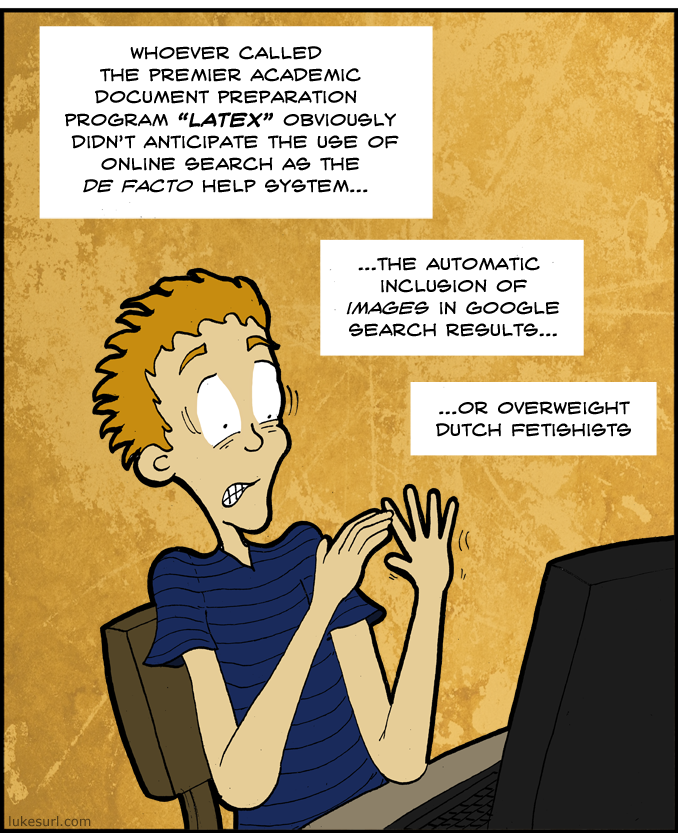
\includegraphics[width=0.75\textwidth]{google_latex.png}
  \caption*{а) Картинка не отцентрирована.}
  \end{minipage}
  \noindent
  \begin{minipage}[t]{.55\textwidth}
  \centering
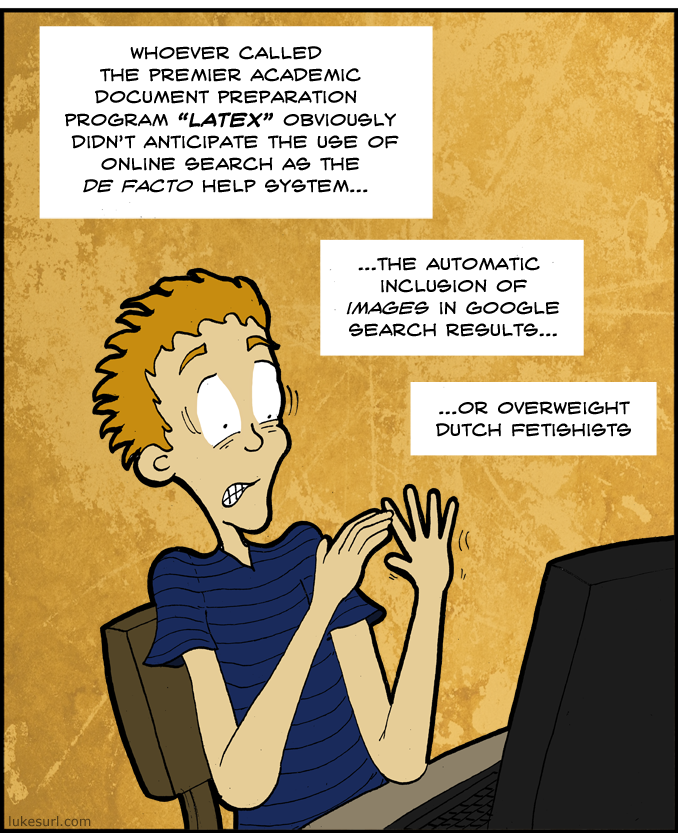
\includegraphics[width=0.75\textwidth]{google_latex.png}
  \caption*{б) Картинка отцентрирована.}
  \end{minipage}
\caption{Пример оформления рисунка.}
\label{fig:example1}
\end{figure}

Внешний рисунок вставляется в картинку командой \texttt{\textbackslash includegraphics}. У неё два аргумента: в квадратных скобках указывается ширина рисунка, в фигурных --- имя файла. Удобнее всего рассчитывать ширину рисунка исходя из актуальной ширины текстового поля, т.е. в долях от константы \texttt{\textbackslash textwidth}. На рисунке~\ref{fig:example1} обе картинки включены с параметром \texttt{0.75\textbackslash textwidth}, но разница существенная, поскольку ширина первой колонки (мини-страницы) составляет 40\% от ширины общего текстового поля, а ширина второй мини-страницы --- 55\%. 

Окружение \texttt{minipage} также формируется с помощью \texttt{\textbackslash begin\{minipage\}[тип выравнивания]\{ширина мини-страницы\}}\dots\texttt{\textbackslash end\{minipage\}}. Тип выравнивания определяет вертикальное выравнивание содержимого мини-страницы и может быть \texttt{c} (центр), \texttt{t} (верх), \texttt{b} (низ)\footnote{Иногда выравнивание по верху и по низу даёт одинаковый результат, однако.}. Ширину мини-страницы тоже удобно описывать как долю от актуальной ширины текстового поля. Если не начинать новый абзац между описаниями мини-страниц, \LaTeX{} попытается выстроить их на одном уровне. Но получится это у него, только если суммарная ширина всех мини-страниц будет чуть-чуть меньше, чем \texttt{\textbackslash textwidth}. Обычно достаточно оставить зазор в 5\% ширины, но в принципе можно подобрать и меньшее значение $\varepsilon$. Например, рисунок~\ref{fig:example1} формирует две параллельные колонки, если заменить в заголовке первой мини-страницы \texttt{.4\textbackslash textwidth} (исходные 40\% ширины) на \texttt{.443\textbackslash textwidth}. 

\subsubsection{Таблицы}

Таблицы оформляются похожим образом. Прежде всего, у достаточно большой таблицы должно быть имя и возможность на неё ссылаться, поэтому такая таблица погружается в окружение \texttt{table}. Это окружение имеет уже знакомую по предыдущим разделам \texttt{begin--end} структуру. В квадратных скобках после \texttt{\textbackslash begin\{table\}} --- рекомендация для \LaTeX, как размещать таблицу относительно страницы. Удобно использовать такую же, как для рисунков, --- \texttt{htb}.

Название рисунка приводится по ГОСТу под ним, а название таблицы --- наоборот, до неё. Поэтому тег \texttt{\textbackslash caption} размещаем на следующей строке после \texttt{\textbackslash begin\{table\}}. Центрирование внутри окружения \texttt{table} также включать обязательно.

Окружение \texttt{tabular} формирует саму таблицу. Заголовок у него такой: \texttt{\textbackslash begin\{tabular\}\{список форматов ячеек\}}. Формат ячейки --- это тип выравнивания её содержимого по ширине (\texttt{r} --- правый край, \texttt{l} --- левый край или \texttt{c} --- середина) и указание, нужны ли вертикальные линии по бокам ячейки. Причём этих линий можно ставить сколько угодно.

Примеры заголовков:
\begin{itemize}
\item \texttt{\textbackslash begin\{tabular\}\{||rllc\}} --- таблица с четырьмя столбцами, первый выровнен по правому краю, последний по центру, остальные по левому краю. Слева от первого столбца двойная вертикальная линия;
\item \texttt{\textbackslash begin\{tabular\}\{l|l|l|lll\}} --- таблица с шестью столбцами, все выровнены по левому краю. Три первых столбца отделены вертикальными линиями.
\end{itemize}

\bigskip

\begin{table}[htb]
\caption{\centering Таблицы, рисунки, листинги.}

\centering\begin{tabular}{|||c|c|c|c||}
\hline\hline
\multirow{ 2}{*}{Особенность} & \multirow{ 2}{*}{Таблицы} & \multirow{ 2}{*}{Рисунки} & \multirow{ 2}{*}{Листинги}\\
& & & \\
\hline
\multirow{ 2}{*}{Окружение} & {\texttt{table}, а внутри}  & \multirow{ 2}{*}{\texttt{figure}} & \texttt{figure}, а внутри \\
&\texttt{tabular} & & \texttt{lstlisting}\\\hline
\multirow{ 3}{*}{Название} & \multirow{ 3}{*}{над таблицей}  & \multirow{ 3}{*}{под рисунком}  & {Аргументом \texttt{caption}}\\
&  &  &  в квадратных скобках \\
& & &{при вызове \texttt{\textbackslash begin\{lstlisting\}}}\\\hline
Центрирование &\multicolumn{2}{c|}{Да} & Нет \\\hline
\multirow{2}{*}{Ссылка} &\multicolumn{2}{c|}{Непосредственно перед} & Аргументом \texttt{label} \\
&\multicolumn{2}{c|}{\texttt{end}--элементом} & {при вызове \texttt{\textbackslash begin\{lstlisting\}}}\\
\hline\hline
\end{tabular}
\label{table:table}
\end{table}

Сама таблица использует команды \&{} --- перейти к ячейке следующего столбца данной строки; и \textbackslash\textbackslash{} --- завершить строку. Если хочется отделить строку линией, после директивы завершения строки дописываем \texttt{\textbackslash hline}. Делаем это столько раз, сколько параллельных линий хотим провести, но нужно учесть, что при такой многократной отрисовке \LaTeX{} коряво оформляет уголки --- точки пересечения дополнительных линий. См.~таблицу~\ref{table:table}. Слияние строк и столбцов в таблице осуществляется командами \texttt{\textbackslash multirow} и \texttt{\textbackslash multicolumn} соответственно. Про их использование можно почитать в мануалах \LaTeX.

\subsubsection{Листинги}

В отличие от рисунка и таблицы, листинг является нестандартным окружением, которое введено с помощью макроса \texttt{lstlisting}. Поэтому его оформление достаточно сильно отличается от предыдущих двух элементов.

Листинг мы тоже помещаем в окружение \texttt{figure} --- не затем чтобы пользоваться ссылкой на него и не затем чтобы именовать его командой \texttt{\textbackslash caption}. Просто если листинг оформлен этим окружением, \LaTeX{} будет пытаться разместить его на странице не как попало, а как можно более аккуратно, как полноценный плавающий объект.

Все атрибуты листинга перечисляются в квадратных скобках после \texttt{\textbackslash begin\{lstlisting\}}. Важнейшие атрибуты:
\begin{itemize}
\item \texttt{caption} --- обязательный атрибут, задающий заголовок;
\item \texttt{label} --- обязательный атрибут, задающий ссылку на листинг;
\item \texttt{language} --- опциональный атрибут, задающий тип разметки ключевых слов (по умолчанию --- Рефал, если разметка не нужна, пишем \texttt{language=\{\}}).
\end{itemize}

Внутри окружения \texttt{lstlisting} \TeX-овские спецсимволы не распознаются (в частности, все обратные слеши в листинге~\ref{lst:kitten} были записаны просто символами), разметка основного текста не применяется, а каждая новая строка начинается как во всех нормальных языках программирования --- не с пустой строки, а просто с символа перевода каретки. Кроме того, автоматически применяется моноширинное начертание и уменьшенный размер шрифта и строки кода нумеруются.

\begin{figure}[!htb]
\begin{lstlisting}[language={C},caption={Пример листинга.},label={lst:kitten}]
int main(){
/* /\---/\ */
/* \ O O / */
/*  \ Y /  */
/*   ---   */
}
\end{lstlisting}
\end{figure}

Кстати, листинг~\ref{lst:kitten} нормоконтроль на ВКР мог не пройти: комментарии в нём выделены зелёным цветом, а цвета разрешены только внутри картинок. Но для курсовой и отчёта по практике выглядит в самый раз.

А ещё листинги можно читать из файла командой \texttt{\textbackslash lstinputlisting[аргументы]\{имя файла\}}. Аргументы здесь такие же, как и у \texttt{lstlisting}. Пример --- Листинг~\ref{lst:scp}.

\begin{figure}[!htb]
\lstinputlisting[caption={Листинг, считанный из файла SCP\_new.ref.},label={lst:scp}]{SCP_new.ref}
\end{figure}

К сожалению, пакет \texttt{listings} плохо взаимодействует с кириллицей, поэтому в тексте листинга не должно встречаться русских букв. 

\subsection{Перекрёстные ссылки}

Это --- второе, ради чего стоит использовать \LaTeX{} (первое --- см. Раздел~\ref{Sect::mathmode}). Система формирования кликабельных ссылок здесь довольно удобна. Большинство объектов, описанных в этом разделе, позволяют создать ссылку на них с помощью команды \texttt{\textbackslash{label}}. Размещать эту команду в окружении надо аккуратно: в теоремах, леммах, примерах и определениях --- сразу после тега \texttt{\textbackslash begin}, без перевода строки; в рисунках и таблицах --- непосредственно перед тегом \texttt{\textbackslash end}. Естественно, можно делать ссылки на разделы и подразделы --- в этом случае \texttt{\textbackslash label} также ставим сразу после тега раздела, без перевода строки.

Имя ссылки может содержать латинские цифры и буквы и указывается в фигурных скобках: \texttt{\textbackslash{label\{имя ссылки\}}}. Принято, что имя ссылки имеет вид \texttt{тип объекта:идентификатор}, где тип объекта --- это \texttt{section}, \texttt{example}, \texttt{figure}, \texttt{table} и т.д. или их сокращения. 

Ссылаемся на объект командой \texttt{\textbackslash ref\{имя ссылки\}}. Обычно требуется скомпилировать исходник дважды, прежде чем корректно расставятся все ссылки.

Ссылка на листинг создаётся только внутри окружения \texttt{lstlisting}. Доказательства по умолчанию не являются объектами, на которые можно делать ссылки.

\section{Математика}\label{Sect::mathmode}

Кто уже оформлял математические тексты, знает, что формулы удобнее набирать не в формате WYSIWYG, а с помощью простого языка программирования. В \LaTeX{} этот язык отлично разработан и после небольшой практики даёт возможность забыть о проблемах с формулами, невыровненными по тексту или отображающимися кракозябрами. В \LaTeX{} есть специальная <<математическая мода>> (режим набора математических формул). Включается математический режим символом \$ или сочетанием \texttt{\textbackslash(}, выключается --- тем же \$ или сочетанием \texttt{\textbackslash)}. 

Вот некоторые особенности режима записи математики:
\begin{itemize}
\item изменены расстояния между символами по умолчанию;
\item обычные пробельные знаки игнорируются (те, что перечислены в списке хаков --- нет);
\item начертание букв по умолчанию --- курсивное, причём оно отличается от курсива в обычном тексте. Цифры в математическом режиме пишутся не курсивом, но в улучшенном начертании. Сравним $blahBLAHblah0987$ и \textit{blahBLAHblah}0987.
\end{itemize}

В математическом режиме есть свои команды для изменения начертания шрифта:
\begin{itemize}
\item \texttt{\textbackslash mathit} --- математический курсив: $\mathit{1234XYZxyz}$;
\item \texttt{\textbackslash mathbf} --- математический полужирный: $\mathbf{1234XYZxyz}$;
\item \texttt{\textbackslash mathtt} --- математический моноширинный: $\mathtt{1234XYZxyz}$; 
\item \texttt{\textbackslash mathrm} --- математический прямой: $\mathrm{1234XYZxyz}$; 
\item \texttt{\textbackslash mathfrak} --- готический: $\mathfrak{1234XYZxyz}$; 
\item \texttt{\textbackslash mathcal} --- каллиграфический: $\mathcal{1234XYZxyz}$; 
\item \texttt{\textbackslash mathbb} --- прозрачный: $\mathbb{1234XYZxyz}$;
\item \texttt{\textbackslash mathscr} --- <<Ralph Smith formal script>>: $\mathscr{1234XYZxyz}$. Здесь под тегом такая же строка, как и в предыдущих примерах, но строчные буквы и цифры просто не отображаются в этом начертании.
\end{itemize}
Как видно, последние три начертания имеет смысл использовать только для заглавных латинских букв, иначе результат может оказаться неожиданным. Впрочем, обычно пользователи именно для них эти начертания и применяют: прозрачным принято записывать значки для числовых множеств, а каллиграфический и RSFS чаще всего используются для обозначения множеств или структур, вводимых автором. Переменные ими не обозначают, впрочем, как и готическим.

\begin{Example}\label{Example:MathFont}
Формула нормального человека: $x_i^2 + y^2_i = \frac{L*\sqrt{S_{i+2}}}{2}$; формула курильщика: $\mathbb{X}_\mathfrak{i}^\mathfrak{2} + \mathcal{Y}^\mathit{2}_\mathtt{i} = \frac{\mathscr{L}*\sqrt{\mathfrak{S}_\mathfrak{i+2}}}{\mathbf{2}}$.
\end{Example} 

Как видно из Примера~\ref{Example:MathFont}, чрезмерно креативное использование альтернативных математических начертаний в тексте не приветствуется. Кроме того, существует негласное правило, что имена переменных чувствительны к начертанию: вот такой $\mathtt{x}$ --- не то же, что такой $\mathbf{x}$, и не то же, что такой $x$. Естественно, если начертания нельзя различить на глаз, например, как в $x$ и $\mathit{x}$ (второй записан курсивом), такие переменные считываются как одинаковые. Но вообще, чтобы не запутаться в начертаниях и именах переменных, удобно пользоваться макросами (см.~Раздел~\ref{Sect::Macros}).

Нормальной кириллицы в математическом режиме нет, но её можно включить в формулу с помощью тега \texttt{\textbackslash text\{...\}}. 

Если формула достойна того, чтобы быть пронумерованной и выключенной из текста (по ГОСТу это одно и то же), тогда используем окружение \texttt{equation}. Включается и выключается оно стандартной \texttt{begin}--\texttt{end} структурой. Ссылка на формулу (тег \texttt{\textbackslash label}) ставится сразу после \texttt{\textbackslash begin\{equation\}}, без переноса строки. Автонумерацию, центрирование и переход в математический режим окружение обеспечит автоматически, так что добавлять знаки долларов не надо.

\begin{Example}\label{Example:MathFont2}
Формула нормального человека: 
\begin{equation}\label{eq:1}
x_i^2 + y^2_i = \frac{L*\sqrt{S_{i+2}}}{2}\,;
\end{equation} 
формула курильщика: 
\begin{equation}\label{eq:2}
\mathbb{X}_\mathfrak{i}^\mathfrak{2} + \mathcal{Y}^\mathit{2}_\mathtt{i} = \frac{\mathscr{L}*\sqrt{\mathfrak{S}_\mathfrak{i+2}}}{\mathbf{2}}
\end{equation}.
\end{Example} 

В формулу~\ref{eq:1} мы были вынуждены добавить точку с запятой, потому что если бы поставили её вне окружения, она бы перенеслась на новую строку, как случилось с формулой~\ref{eq:2}. На то она и формула курильщика. Также из-за манеры математического режима изменять расстояния между символами пришлось добавить принудительный короткий пробел \texttt{\textbackslash ,} перед точкой с запятой. 

\subsection{Часто используемые фишки}
\subsubsection{Нижние и верхние индексы}

Режим нижних и верхних индексов работает только в математическом режиме. Нижний индекс --- это символ или группа символов в фигурных скобках после знака подчёркивания \_; верхний индекс --- то же после крышки \^{}.

Если индекс состоит больше чем из одного символа, про фигурные скобки забывать нельзя, иначе все символы, кроме первого, будут уже не считаться индексом. Например, если $x$ хочется снабдить сложным индексом $i+k*m$, то записав это вот так: $x_i+k*m$, получим совсем не то, что нужно. Правильно: $x_{i+k*m}$.

Нижние и верхние индексы могут быть использованы внутри индексов и образовывать какие угодно сочетания, например: $A^{B^{B^{B^B}}_{C^D}}_{E_{F_G}}$. С каждым новым уровнем индексов вплоть до третьего размер шрифта уменьшается, а дальше остаётся постоянным.

\subsubsection{Логические и теоретико-множественные формулы}

С ними довольно часто приходится иметь дело, поэтому здесь будут перечислены основные команды для записи логики:
\begin{itemize}
\item \texttt{\textbackslash forall} --- знак всеобщности $\forall$;
\item \texttt{\textbackslash exists} --- знак существования $\exists$;
\item \texttt{\textbackslash wedge} или \texttt{\textbackslash \&} --- конъюнкция $\wedge$ или $\&$;
\item \texttt{\textbackslash vee} --- дизъюнкция $\vee$;
\item \texttt{\textbackslash Rightarrow} --- импликация $\Rightarrow$, не путаем с \texttt{\textbackslash rightarrow} --- стрелкой $\rightarrow$;
\item \texttt{\textbackslash neg} --- отрицание $\neg$;
\item \texttt{\textbackslash subseteq} --- нестрогое отношение подмножества $\subseteq$;
\item \texttt{\textbackslash subset} --- строгое отношение подмножества $\subset$;
\item \texttt{\textbackslash cup} --- пересечение множеств $\cup$;
\item \texttt{\textbackslash cap} --- объединение $\cap$;
\item \texttt{\textbackslash backslash} --- разность множеств $\backslash$ --- в обычном тексте этот тег работать не будет;
\item \texttt{\textbackslash in} --- знак принадлежности $\in$;
\item \texttt{\textbackslash notin} --- знак непринадлежности $\notin$.
\end{itemize}

Далее мы в тему специальных символов не углубляемся, они перечислены в справочниках по \LaTeX.

\subsection{Макросы}\label{Sect::Macros}

Особенности математического режима таковы, что для красивого ввода имени, состоящего из нескольких латинских букв, приходится использовать хаки. Сравним $BUgs$ и $BU\hspace{-.3ex}gs$ --- в первом имени все четыре буквы записаны просто подряд, и оно выглядит как последовательность из двух двухбуквенных имён; во втором между $U$ и $g$ добавлен хак \texttt{\textbackslash hspace\{-.3ex\}} и оно уже выглядит нормально. Однако добавлять такие хаки всюду по тексту записки --- то ещё удовольствие, к тому же где-нибудь да он забудется. Чтобы минимизировать опечатки в идентификаторах, используемых в формулах, и сделать их внесение в текст менее трудозатратным, можно применить механизм макросов.

Для определения нового макроса--имени нужно в преамбулу документа, желательно после всех прочих записей в преамбуле, добавить команду \texttt{\textbackslash newcommand\{имя команды, начинается с бэкслэша\}\{тело команды\}}. После этого тело команды будет инлайниться в код вместо указанного имени. 

\begin{Example}
Допустим, в преамбулу добавлена директива:

\centering{\texttt{\textbackslash newcommand\{\textbackslash bug\}\{\textbackslash mathbf\{B\textbackslash hspace\{-.2ex\}U\textbackslash hspace\{-.2ex\}G\} \textbackslash hspace\{.1ex\}\textbackslash mathrm\{A\textbackslash hspace\{-.2ex\}G\textbackslash hspace\{-.2ex\}A\}\}}.}

\vspace{-1.5ex}

\justify Она будет рисовать идентификатор $\mathbf{B\hspace{-0.2ex}U\hspace{-0.2ex}G}\hspace{0.1ex}\mathrm{A\hspace{-0.2ex}G\hspace{-0.2ex}A}$ везде, где встретит тег \texttt{\textbackslash bug}, правда, вне математического режима скомпилируется с ошибкой, поскольку тело макроса использует команды, специфические для него. Теперь, если мы захотим заменить этот идентификатор, например, на $\bot$, это делается простейшей заменой макроса на \texttt{\textbackslash newcommand\{\textbackslash bug\}\{\textbackslash bot\}}, и всё, дальше по тексту можно не проверять, все ли нужные идентификаторы заменились, и не заменилось ли что-то лишнее. Только помним, что если исходный идентификатор годился для математического режима, то его замена тоже должна использовать команды этого же режима.
\end{Example}

\section{Подключение и сборка библиографии}

Библиография готовится в отдельном файле с расширением \texttt{bib} и использует ГОСТовский стиль \texttt{ugost2008s.bst}. \texttt{bib}-файл --- это база данных, где хранятся записи об использованных источниках. Конкретное имя этого файла указывается командой \texttt{\textbackslash bibliography}. В нашем случае это \texttt{\textbackslash bibliography\{biblio\}}.

Порядок записей в \texttt{bib}-файле может быть какой угодно, как и полей в них --- \LaTeX{} упорядочит всё как надо сам. Для сборки библиографии запустить \texttt{bibtex} и скомпилировать исходник дважды. Если ссылки всё ещё отображаются некорректно --- возможно, \LaTeX{} собрал информацию для вспомогательных файлов ещё не полностью, и рекомпиляция может решить эту проблему.

На примере элемента библиографии в Листинге~\ref{lst:bib} посмотрим на структуру записи. 

\begin{figure}[!htb]
\begin{lstlisting}[language={TeX},caption={Пример элемента библиографии},label={lst:bib}]
@article{Vybegallo,
 author = {Vybegallo, A.A. and A.A. Vybegallo},
 title = {About Reverse Analysis of Gorilla Language},
 journal = {Vestnik NII CHAVO},
 year = {2222},
 pages = {1--111},
 number = {0},
 language = {english}
}
\end{lstlisting}
\end{figure}

На результат можно полюбоваться в списке использованных источников~\cite{Vybegallo}. Имя ссылки --- это самое первое поле, сразу после типа записи. Здесь имя \texttt{Vybegallo}. Чтобы процитировать элемент библиографии с таким именем в тексте, пишем \texttt{\textbackslash cite\{Vybegallo\}}. Цитирование указывается в конце текстового отрезка, к которому оно относится. Желательно применять неразрывный пробел для связи команды \texttt{cite} с последним словом, ему предшествующим.

Отметим некоторые детали:
\begin{itemize}
\item не забываем экранировать служебные символы --- библиография не листинг;
\item после каждой записи, кроме последней, ставится запятая;
\item если вы не уверены, что парсер обработает запись однозначно, лучше заключить её в фигурные скобки;
\item при записи диапазона страниц используем короткое тире --- записывается так -{}-;
\item если источник опубликован на английском языке, язык нужно указать, тогда как русский указывать не обязательно;
\item если в имени автора инициалы идут после его фамилии, отделяем их от фамилии запятой;
\item если автор не один, перечисляем их через служебное слово \texttt{and} (без выделения запятыми). 
\end{itemize}

\LaTeX{} неплохо распознаёт фамилию и инициалы. Как видно по ссылке~\cite{Vybegallo}, библиографический стиль поместил фамилию Амвросия Амвруазовича перед именем--отчеством, хотя во втором случае имя--отчество предшествовали фамилии. 

Обычная для технических текстов информация с датой обращения к электронному ресурсу помещается в поле \texttt{annote}. Она автоматически будет заключена в круглые скобки. 

Библиографическую информацию об источниках, опубликованных в индексируемых журналах, почти всегда можно найти на открытых страницах в формате, подходящем для базы данных \texttt{bib}. Современные зарубежные статьи чаще всего есть на \url{dblp.org}, русскоязычные --- на \url{mathnet.ru} (правда, там по умолчанию используется AMSbib-формат, чуть-чуть отличный от стандартного). На elibrary скачать bibtex-образец нельзя, но обычно есть ссылка на doi, которая может вывести на страницу, где он есть.

\section{Чтение лога и тестирование}

В логе (файл \texttt{.log}) можно посмотреть сообщения об ошибках, мешающих собрать документ, и о предупреждениях. Многие из последних --- издержки взаимодействия разных пакетов. Перечислим только те, которые со стилем не связаны.

\begin{enumerate}
\item Если предупреждение имеет вид \texttt{Citation ... on page ... undefined} или \texttt{Reference ... on page ... undefined}, значит, есть опечатка в цитировании или обращении к ссылке.
\item Если в логе встретились слова \texttt{Underfull} или \texttt{Overfull}, это указывает на то, что текст не соответствует установленному формату полей. В целом, на недополнения не стоит обращать особенного внимания, за исключением случая, когда разреженность текста сильно бросается в глаза. Переполнения лучше исключить, кроме того, которое в болванке есть на титульной странице (эмблема МГТУ чуть-чуть вылазит влево за поле прозрачным фоном).
\end{enumerate}

После того, как ошибок, потерянных ссылок и критических переполнений в логе не будет, можно убедиться, что \LaTeX{} не слишком сильно изменил параметры основного шрифта в документе. Для этого открываем Word или его аналог и копируем кусок основного текста из свёрстванного pdf-документа. Имя шрифта должно быть из семейства  Tempora (это бесплатная версия times, содержащая курсивное и полужирное начертания дли кириллицы), и обязательно 14-го размера.

 \anonsection{ЗАКЛЮЧЕНИЕ} %\anonsection{Заключение}

Этот исходник подготовлен с помощью системы \LaTeX{} на базе приложения к положению о нормоконтроле МГТУ им. Н.\,Э. Баумана~\cite{normcor}. Подробно про возможности языка разметки можно почитать в обстоятельном труде Львовского~\cite{LaTeX2e}, а большинство мелких вопросов решается поиском, например, в соответствующем разделе StackExchange~\cite{stackexchange}. Запросы в гугле по слову \texttt{'latex'} лучше формулировать как можно конкретнее (см.~Рисунок~\ref{fig:example1}). 

Установка и настройка \LaTeX{} --- не самое приятное занятие, зато реакция преподавателей на результат может быть очень приятной (см. Рисунок~\ref{fig::thesis}). Конечно, всё это имеет смысл, если в вашей работе много формул и перекрёстных ссылок. Простой текст легче набивать в WYSIWYG-редакторе.

\renewcommand\refname{СПИСОК ИСПОЛЬЗОВАННЫХ ИСТОЧНИКОВ}
% Список литературы
\clearpage
\bibliographystyle{ugost2008s}  %utf8gost71u.bst} %utf8gost705u} %gost2008s}
{\catcode`"\active\def"{\relax}
\addcontentsline{toc}{section}{\protect\numberline{}\refname}%
\bibliography{biblio} %здесь ничего не меняем, кроме, возможно, имени bib-файла
}
\newpage
\settocdepth{section}
\anonsection{ПРИЛОЖЕНИЕ А}

\vspace{-20pt}
\begin{figure}[!htb]\centering

\includegraphics[width=0.5\textwidth]{thesis_latex.jpg}
\caption{Что было бы, если бы записки принимались на любом языке программирования.}
\label{fig::thesis}
\end{figure}
\end{document}
